\chapter{Encoding the Sequent Calculus}
\label{chap:sequentcalculus}

Jape is, at bottom, a backwards-reasoning proof editor working on a tree of sequents. It is therefore no surprise that it is exceptionally straightforward to encode the sequent calculus in Jape. We describe in this chapter the encoding of the multiple-conclusion sequent calculus in the file \texttt{examples/sequent\_calculus/MCS.jt} and the files it references. 

The rules we use, and the examples, were borrowed from Roy Dyckhoff's excellent MacLogic (an inspiring precursor of Jape). This encoding draws heavily on the single-conclusion sequent calculus encoding (see \texttt{examples/SCS.jt}), developed jointly by Bernard Sufrin and myself in the early days of Jape, so `we' is Bernard and me. The encoding is quite old, and the segmentation into files is somewhat arbitrary.

\begin{table}
\centering
\caption{The \texttt{axiom} rule}
\label{tab:seqcalculusaxiom}
\vstrut{20pt}
$\infer[\reason{axiom}]
       {\Gamma,A |- A,\Delta }
       {}$ 
\end{table}

\begin{table}
\centering
\caption{Introduction to the right of the turnstile (⊦... rules)}
\label{tab:sequentleftrules}
\vstrut{30pt}
$\infer[\reason{⊦∧}]
       {\Gamma  |- A@B,\Delta }
       {\Gamma  |- A,\Delta & \Gamma  |- B,\Delta }$
\qquad\vstrut{30pt}
$\infer[\reason{⊦→}]
       {\Gamma  |- A->B,\Delta }
       {\Gamma,A |- B,\Delta }$
\qquad\vstrut{30pt}
$\infer[\reason{⊦∨}]
       {\Gamma  |- A|B,\Delta }
       {\Gamma  |- A,B,\Delta }$
\qquad\vstrut{30pt}
$\infer[\reason{⊦¬ }]
       {\Gamma  |- !A,\Delta }
       {\Gamma,A |- \Delta }$ 
\qquad\vstrut{30pt}
$\infer[\reason{⊦≡}]
       {\Gamma |- A\equiv B, \Delta }
       {\Gamma |- A->B, \Delta & \Gamma |- B->A, \Delta }$
\qquad\vstrut{30pt}
$\infer[\reason{(fresh $m$) ⊦∀}]
       {\Gamma  |- @*x.A(x),\Delta }
       {\Gamma  |- A(m),\Delta }$
\qquad\vstrut{30pt}
$\infer[\reason{⊦∃}]
       {\Gamma  |-|*x.A(x),\Delta }
       {\Gamma  |- A(B),\Delta }$
\end{table}


\begin{table}
\centering
\caption{Introduction to the left of the turnstile (...⊦ rules)}
\label{tab:sequentrightrules}
$\infer[\reason{∧⊦}]
       {\Gamma,A@B |- \Delta }
       {\Gamma,A,B |- \Delta }$
\qquad\vstrut{30pt}
$\infer[\reason{→⊦}]
       {\Gamma,A->B |- \Delta }
       {\Gamma  |- A,\Delta & \Gamma,B |- \Delta }$
\qquad\vstrut{30pt}
$\infer[\reason{∨⊦}]
       {\Gamma,A|B |- \Delta }
       {\Gamma,A |- \Delta & \Gamma,B |- \Delta }$
\qquad\vstrut{30pt}
$\infer[\reason{¬⊦}]
       {\Gamma,!A |- \Delta }
       {\Gamma  |- A,\Delta }$ 
\qquad\vstrut{30pt}
$\infer[\reason{≡⊦}]
       {\Gamma,A->B,B->A|-C}
       {\Gamma,A\equiv B |-C}$
\qquad\vstrut{30pt}
$\infer[\reason{∀⊦}]
       {\Gamma,@*x.A(x)  |- \Delta }
       {\Gamma,A(B)  |- \Delta }$
\qquad\vstrut{30pt}
$\infer[\reason{(fresh $m$) ∃⊦}]
       {\Gamma,|*x.A(x)  |- \Delta }
       {\Gamma,A( m)  |- \Delta }$
\end{table}


\begin{table}
\centering
\caption{Structural rules}
\label{tab:sequentstructuralrules}
$\infer[\reason{cut}]
       {\Gamma  |- \Delta }
       {\Gamma  |- B,\Delta & \Gamma,B |- \Delta }$
\qquad\vstrut{30pt}
$\infer[\reason{⊦ weaken}]
       {\Gamma  |- A,\Delta }
       {\Gamma  |- \Delta }$
\qquad\vstrut{30pt}
$\infer[\reason{⊦ contract}]
       {\Gamma  |- A,\Delta }
       {\Gamma  |- A,A,\Delta }$
\qquad\vstrut{30pt}
$\infer[\reason{weaken ⊦}]
       {\Gamma,A |- \Delta }
       {\Gamma  |- \Delta }$
\qquad\vstrut{30pt}
$\infer[\reason{contract ⊦}]
       {\Gamma,A |- \Delta }
       {\Gamma,A,A |- \Delta }$
\end{table}

\begin{table}
\centering
\caption{Modified quantifier rules}
\label{tab:seqcalculusquantifierrules}
$\infer[\reason{(fresh $m$) ⊦∀}]
       {\Gamma  |- @*x.A,\Delta }
       {\Gamma  |- A[x\backslash m],\Delta }$
\qquad\vstrut{30pt}
$\infer[\reason{⊦∃}]
       {\Gamma  |- |*x.A,\Delta }
       {\Gamma  |- A[x\backslash B],\Delta }$
\qquad\vstrut{30pt}
$\infer[\reason{∀⊦}]
       {\Gamma,@*x.A |- \Delta }
       {\Gamma,A[x\backslash B]  |- \Delta }$
\qquad\vstrut{30pt}
$\infer[\reason{(fresh $m$) ∃⊦}]
       {\Gamma,|*x.A |- \Delta }
       {\Gamma,A[x\backslash m]  |- \Delta }$\vstrut{30pt}
\end{table}

\section{The inference rules of the (multiple-conclusion) Sequent Calculus}

We have encoded a standard version of the sequent calculus. By making our left- and right-hand sides \textit{bags} (aka multisets) of formulae we have avoided the need for exchange rules; by allowing the axiom rule to ignore unnecessary hypotheses and conclusions we have avoided the need to use weakening rules in almost every case and/or to describe context-splitting rules. See \chapref{sequentvariations} for an alternative treatment of quantifiers and variables and for Jape's treatment of context-splitting (multiplicative) rules.

The rules, given in tables \ref{tab:seqcalculusaxiom}, \ref{tab:sequentleftrules}, \ref{tab:sequentrightrules} and \ref{tab:sequentstructuralrules}, are additive --- that is, don't split their left- or right-hand side contexts working backwards. Multiplicative (context-splitting) rules are harder to use in a backwards reasoning tool, because either the tool must force the user to decide how to split the context before the rule is applied or else it must provide machinery to allow the decision to be deferred (Jape chooses deferral: see \chapref{sequentvariations}). In this encoding, the fact that the \textit{axiom} rule ignores unnecessary hypothesis and conclusion formulae makes context-splitting on either side unnecessary.

Because Jape interprets predicate notation as shorthand for substitution, the \textit{actual} quantifier rules use substitution. \Tabref{seqcalculusquantifierrules} shows the rules which Jape employs, translating the originals on input. The difference need hardly detain us: there are no additional provisos, and no substitution-matching is required. In this logic at least, it's easy to believe that Jape manipulates predicate notation directly.


\section{Syntax description (\texttt{sequent\_syntax.j})}

We begin with a couple of variable initialisations:\footnote{The syntactic form we use is that of an assignment to a variable. The \texttt{interpretpredicates} variable can only be altered when the store of rules and variables is empty, so in practice it behaves as a parameter.}
\begin{quote}\tt\small
INITIALISE interpretpredicates true \\
INITIALISE displaystyle tree
\end{quote}
This ensures that juxtapositions are interpreted as predicate application, and that we see the proofs as trees.

We use names starting with A, B, C, D, P, Q, R and S in rules and conjectures to stand for any formula; we use names starting with u, v, w, x, y, z. m or n to stand for any variable. Names starting with Γ or Δ stand for bags (multisets) of formulae\footnote{Note that now there are no commas in these lists of identifier prefixes: I have eliminated use of comma as a separator in the paragraph language. See \appxref{paraformlang} for more details}.

\begin{quote}\tt\small
CLASS BAG Γ ∆ \\
CLASS FORMULA A B C D P Q R S \\
CLASS VARIABLE u v w x y z m n
\end{quote}

These directives also cover unknowns: an unknown which starts $\_A$ will unify with any formula, but one which starts $\_z$ will only unify with a variable or a similar unknown.

Quantifier formulae are, like if-then-else in most programming languages, bracketed without a final closing bracket:
\begin{quote}\tt\small
LEFTFIX 20              ∀ .\\
LEFTFIX 20              ∃ .
\end{quote}
The connectives are defined as operators with particular \emph{binding power} and \emph{binding direction}:
\begin{quote}\tt\small
INFIX           100L            ≡\\
INFIX           110R            →\\
INFIX           150L            ∧\\
INFIX           160L            ∨\\
PREFIX          200             ¬
\end{quote}
The relative binding power of juxtaposition and substitutions are defined:
\begin{quote}\tt\small
JUXTFIX         300 \\
SUBSTFIX        400 
\end{quote}
Working from the bottom, this defines substitution forms as the most binding, then juxtaposition. Next comes ¬ defined as a prefix operator, then the binary connectives (all but → are defined to be left-associative, while → is right-associative). Finally two special bracketed forms are defined, with the lowest syntactic priority. These definitions allow us to write:
\var{prim,f1,f2}
\begin{itemize}
\item $!\<prim>$, where $\<prim>$ is an atomic formula, a substitution or a juxtaposition (see \appxref{paraformlang});

\item $\<f1>|\<f2>$, $\<f1>@\<f2>$ or $\<f1>->\<f2>$ with the interpretation that ∨ `operators' have priority over ∧, and both have priority over →;

\item \ensuremath{@*} $\<f1>$. $\<f2>$ and \ensuremath{|*} $\<f1>$ . $\<f2>$.
\end{itemize}

Note that the leftfix patterns don't constrain you to write ∀\textit{variable}.\textit{formula}: that comes later.

Because there is no closing bracket, formulae constructed with \textsc{leftfix} bracketing are liable to have a visually ambiguous interpretation, so Jape demands that \textsc{leftfix}-brackets aren't used like ordinary brackets: that is, you can't write things like $f1@@*x.f2@f3$ : you have to write instead either $f1@(@*x.f2@f3) $ or $f1@(@*x.f2) @f3$ .

The binding structures are given by pattern:
\begin{quote}\tt\small
BIND    x SCOPE P IN ∃x . P\\
BIND    x SCOPE P IN ∀x . P
\end{quote}
Any formula which matches one of these patterns is recognised as a binding formula --- any variable in place of \textit{x}, any formula, including another binding formula, in place of $P$. Near matches aren't allowed, so the constraint to write \textit{quantifier} \textit{variable}. \textit{formula} is enforced.

Note that this defines only single-variable bindings. Jape has no means at present of defining families of binding structures, except by exhaustively listing them --- for example, you might give \textsc{bind} directives which describe the structure of \ensuremath{@*}\textit{x},y.$E$, \ensuremath{@*}\textit{x},\textit{y},$z$.$E$ and so on as we do in later chapters. But then you would find that Jape has no means of defining families of inference rules which work across the different kinds of bindings you can define, and you would have to separately define the rules --- one for \ensuremath{@*}\textit{x}.$E$, another for \ensuremath{@*}\textit{x},y.$E$, another for \ensuremath{@*}\textit{x},\textit{y},$z$.$E$ and so on.

\section{Encoding the inference rules (\texttt{MCS\_rules.j})}

Our sequents have bags of formulae on either side:

\begin{quote}\tt\small
SEQUENT IS BAG ⊦ BAG
\end{quote}

Jape is designed to make the encoding of inference rules as transparent and straightforward as possible. In principle all you have to do is to linearise the normal description of a rule, giving its name, its provisos, its antecedents and its consequent. Writing \{... \} for optional inclusion and \{... \}* for repeated optional inclusion, the syntax of a \textsc{rule} directive is

\begin{tabular}{lll}
\textsc{rule} & \{ \textit{name} \} & --- \textit{rule name}\\
 & \{ (\textit{parameter} \{, \textit{parameter} \}*) \} & --- \textit{parameters}\\
 & \{ \textsc{where} \textit{proviso} \{\textsc{and} \textit{proviso}\}* \} & --- \textit{provisos}\\
 & \{ \textsc{is} \}\\
 & \{ \textsc{from} \textit{sequent} \{\textsc{and} \textit{sequent}\}* \} & --- \textit{antecedents}\\
 & \textsc{infer} \textit{sequent} & --- \textit{consequent}
\end{tabular}

Nearly everything is optional, but you have to put in enough reserved words to make it clear where each section begins and ends. If you leave the name out, the name is taken to be the consequent itself. Where the name of a rule isn't an identifier --- if it is ⊦∧, for example --- it is necessary to enclose it in quotation marks. The parameters are each an identifier or the word \textsc{object} followed by an identifier. Parameters in a rule definition control the process of instantiation and the treatment of argument formulae provided via text-selection and/or tactics.

The rules are:
\begin{quote}\tt\small
RULE    axiom(A)                                        INFER Γ,A ⊢ A,∆\\
RULE    "⊢∧"        FROM Γ ⊢ A,∆ AND Γ ⊢ B,∆    INFER Γ ⊢ A∧B,∆\\
RULE    "∧⊢"        FROM Γ,A,B ⊢ ∆                INFER Γ,A∧B ⊢ ∆\\
RULE    "⊢∨"        FROM Γ ⊢ A,B,∆                 INFER Γ ⊢ A∨B,∆\\
RULE    "∨⊢"        FROM Γ,A ⊢ ∆ AND Γ,B ⊢ ∆    INFER Γ,A∨B ⊢ ∆\\
RULE    "⊢¬"        FROM Γ,A ⊢ ∆                   INFER Γ ⊢ ¬A,∆\\
RULE    "¬⊢"        FROM Γ ⊢ A,∆                   INFER Γ,¬A ⊢ ∆\\
RULE    "⊢→"        FROM Γ,A ⊢ B,∆                 INFER Γ ⊢ A→B,∆\\
RULE    "→⊢"        FROM Γ ⊢ A,∆ AND Γ,B ⊢ ∆    INFER Γ,A→B ⊢ ∆\\
RULE    "⊢≡"        FROM Γ ⊢ A→B,∆ AND Γ ⊢ B→A,∆    INFER Γ ⊢ A≡B,∆\\
RULE    "≡⊢"        FROM Γ, A→B, B→A ⊢ ∆         INFER Γ,A≡B ⊢ ∆\\
RULE    "⊢∀"(OBJECT m) WHERE FRESH m\\
\tab                     FROM Γ ⊢ A(m),∆                INFER Γ ⊢ ∀x.A(x),∆\\
RULE    "∀⊢"(B)     FROM Γ, A(B) ⊢ ∆               INFER Γ,∀x.A(x) ⊢ ∆\\
RULE    "⊢∃"(B)     FROM Γ ⊢ A(B),∆                INFER Γ ⊢ ∃x.A(x),∆\\
RULE    "∃⊢"(OBJECT m) WHERE FRESH m\\
\tab                     FROM  Γ,A(m) ⊢ ∆               INFER Γ, ∃x.A(x) ⊢ ∆\\
RULE    cut(A)  FROM Γ ⊢ A,∆ AND Γ,A ⊢ ∆          INFER Γ ⊢ ∆\\
RULE    "weaken⊢"(A)    FROM Γ ⊢ ∆                  INFER Γ,A ⊢ ∆\\
RULE    "⊢weaken"(A)    FROM Γ ⊢ ∆                  INFER Γ ⊢ A,∆\\
RULE    "contract⊢"(A)  FROM Γ, A, A ⊢ ∆            INFER Γ, A ⊢ ∆\\
RULE    "⊢contract"(A)  FROM Γ ⊢ A,A,∆              INFER Γ ⊢ A,∆
\end{quote}

The structural rules are given their proper r\^{o}les:

\begin{quote}\tt\small
STRUCTURERULE CUT                   cut\\
STRUCTURERULE LEFTWEAKEN        "weaken⊢"\\
STRUCTURERULE RIGHTWEAKEN       "⊢weaken"
\end{quote}

\section{Automatic application of rules}

It is possible to require Jape to try a tactic at the end of each proof step --- that is, after producing the effects demanded by the user. You can make it apply the tactic in one of two ways: the \textsc{automatch} directive requires that the tactic works without introducing or eliminating any unknowns from the proof tree, and without introducing or eliminating any provisos; the \textsc{autounify} directive doesn't have any of those constraints. With either directive, a rule within the tactic is not applied if there is more than one distinct possible result.

In the sequent calculus it is reasonable to apply \textit{axiom} whenever possible, but because it would always be applicable whenever a conclusion or a hypothesis was a single unknown, it's prudent to restrict ourselves to applications which succeed by identical match, and we therefore include
\begin{quote}\tt\small
AUTOMATCH axiom
\end{quote}

\section{Automatic selection of rules}

When the user double-clicks on, or `hits', a formula, the logic designer can provide that a tactic is automatically applied. The choice of tactic is made by pattern-matching and depends on whether it is a hypothesis or a conclusion that is hit. If there isn't an applicable tactic, Jape puts up an error alert.

Description of a `hit' and what to do about it is given by one of the directives
\begin{quote}
\textsc{conchit\tab }\textit{pattern} \textsc{is} \textit{tactic}\\
\textsc{hyphit\tab }\textit{pattern} \textsc{is} \textit{tactic}
\end{quote}

The pattern is matched --- by one-way matching, not unification --- to the formulae which have been selected and hit. It can be as follows:
\begin{itemize}
\item \textit{hypothesis} \texttt{<}entails\texttt{>} \textit{conclusion}, in which case the user must select (click) one of the two and hit (double-click) the other;
\item \textit{hypothesis} \texttt{<}entails\texttt{>} --- only in \textsc{hyphit} --- in which case the user must hit a hypothesis without selecting a conclusion;
\item \textit{conclusion} or \texttt{<}entails\texttt{>} \textit{conclusion} --- only in \textsc{conchit} --- in which case the user must hit a conclusion without selecting a hypothesis.
\end{itemize}


In the sequent calculus we can automatically invoke a tactic when any formula is hit. First, we can invoke a right rule when any conclusion is hit, provided that the user hasn't confused the issue by selecting a hypothesis as well:
\begin{quote}\tt\small
CONCHIT ⊢ B∧C   IS "⊢∧"\\
CONCHIT ⊢ B∨C   IS "⊢∨"      \\
CONCHIT ⊢ B→C   IS "⊢→"\\
CONCHIT ⊢ ¬B        IS "⊢¬"       \\
CONCHIT ⊢ B≡C   IS "⊢≡"     \\
CONCHIT ⊢ ∀x.B  IS "⊢∀"  \\
CONCHIT ⊢ ∃x.B  IS "⊢∃"  
\end{quote}

We can automatically invoke \textit{axiom} if the user hits a hypothesis having selected an identical conclusion:
\begin{quote}\tt\small
HYPHIT  A ⊢ A   IS axiom       
\end{quote}

We can automatically invoke a left rule if the user hits a hypothesis without having selected a conclusion:
\begin{quote}\tt\small
HYPHIT  A→B ⊢   IS "→⊢"        \\
HYPHIT  A∨B ⊢   IS "∨⊢"\\
HYPHIT  A∧B ⊢   IS "∧⊢"    \\
HYPHIT  ¬A ⊢        IS "¬⊢"    \\
HYPHIT  A≡B ⊢   IS "≡⊢"    \\
HYPHIT  ∀x.A ⊢  IS "∀⊢"\\
HYPHIT  ∃x.A ⊢  IS "∃⊢"
\end{quote}

\section{Menus}

Jape automatically provides some system menus, whose content is not described here. All other menus and panels are produced under the control of the encoder.

\subsection{The Rules menu}


To describe a menu you give its title and its contents. Each entry in the menu has a label --- which the user sees --- and a Jape tactic --- which is transmitted to the Jape engine when the entry is selected. A rule name is the simplest form of Jape tactic, and in this logic that is all that we need:
\begin{quote}\tt\small
MENU Rules IS\\
\tab   ENTRY axiom\\
\tab   SEPARATOR\\
\tab   ENTRY "∧⊢"\\
\tab   ENTRY "∨⊢"\\
\tab   ENTRY "→⊢"\\
\tab   ENTRY "¬⊢"\\
\tab   ENTRY "≡⊢"\\
\tab   ENTRY "∀⊢"\\
\tab   ENTRY "∃⊢"\\
\tab   SEPARATOR\\
\tab   ENTRY "⊢∧"\\
\tab   ENTRY "⊢∨"\\
\tab   ENTRY "⊢→"\\
\tab   ENTRY "⊢¬"\\
\tab   ENTRY "⊢≡"\\
\tab   ENTRY "⊢∀"\\
\tab   ENTRY "⊢∃"\\
\tab   SEPARATOR\\
\tab   ENTRY cut   \\
\tab   ENTRY "weaken⊢"\\
\tab   ENTRY "⊢weaken"\\
\tab   ENTRY "contract⊢"\\
\tab   ENTRY "⊢contract"\\
END
\end{quote}

This produces a menu in which every label is the name of a rule, and every command a tactic of the same name. Jape allows us to save effort by defining the rules within the menu description. If we had written
\begin{quote}\tt\small
MENU Rules IS\\
\tab RULE axiom\tab INFER A ⊦ A\\
\tab SEPARATOR\\
\tab RULE "⊦∧"\tab FROM ⊦ A AND ⊦ B\tab INFER ⊦ A∧B\\
\tab ...\\
END
\end{quote}
then it would have produced exactly the same menu.

\section{Conjectures (\texttt{sequent\_problems.j})}

The primary object of using Jape is to prove theorems. You can state conjectures in text commands composed from the keyboard (after pressing the New\dots button on a conjectures panel), but it is more normal to state them in a logic-encoding file.

Panels in Jape have lists of entries and buttons. A \textsc{conjecturepanel} automatically includes buttons labelled New\dots, Prove and Show Proof, and has a default Apply button if the user defines no buttons at all. In the case of the sequent calculus we can use a straightforward \textsc{conjecturepanel} with a default Apply button to hold all the problems which we want to display to the user. 

A conjecture can be stated in a \textsc{theorem} directive which gives its name, its parameter identifiers and provisos if any, and the sequent which is the theorem itself. The effect is to put a conjecture with that name into the `tactic store', from which it can be retrieved in order to prove it, to apply it during a proof, or to review its proof.

Two conjectures are stated in this way in \texttt{MCS.jt}. We state the panel into which we want to put the conjectures, and give the conjectures themselves. 
\begin{quote}\tt\small
CONJECTUREPANEL "Conjectures"\\
\tab THEOREM   modusponens IS A, A→B ⊢ B\\
\tab THEOREM   contradiction   IS A, ¬A ⊢ \\
END
\end{quote}
These directives are cumulative: the conjectures are added to the panel unless there are already entries with the same name, in which case these replace the previous versions.

Because this logic includes a cut rule and both a left and a right weakening rule, the contradiction theorem can be applied, once proved, to any sequent which has a formula and its negation in its hypotheses. It could even be applied automatically via \textsc{automatch}, though we haven't done that in this encoding.

Interpretation of parameter identifiers and provisos in a \textsc{theorem} directive is the same as for inference rules. 

The rest of the conjectures are given in \texttt{sequent\_problems.j} without names, so that they appear in the panel under names generated from their sequent:
\begin{quote}\tt\small
CONJECTUREPANEL "Conjectures"\\
\tab THEOREM INFER P→(Q→R)                         ⊢ (P→Q)→(P→R)\\
\tab THEOREM INFER P→(Q→R), Q                      ⊢ P→R\\
\tab THEOREM INFER R→S                              ⊢ (P→R) → (P→S)\\
\tab THEOREM INFER P→(P→Q)                         ⊢ P→Q\\
\tab THEOREM INFER P                                 ⊢ Q→(P∧Q)\\
\tab \dots  \\
\\
\tab THEOREM INFER ∀x.¬Q(x),  P→(∀x.Q(x))                              ⊢ ¬P\\
\tab THEOREM WHERE x NOTIN P INFER \\
\tab \tab P∨¬P, ∀x.P→Q(x), ∀x.¬P→Q(x)     ⊢ ∀x.Q(x)\\
\tab THEOREM INFER R∨¬R, ∀x.R→S(x), ∀x.¬R→S(x)                     ⊢ ∀x.S(x)\\
\tab THEOREM INFER ∀x.P(x)→Q(x), ∀x.Q(x)→R(x)                          ⊢ ∀x.P(x)→R(x)\\
\tab THEOREM INFER \\
\tab \tab ∀x.P(x)→R(x), ∀x.Q(x)→ ¬R(x) ⊢ ∀x.(P(x)→¬Q(x))∧(Q(x)→¬P(x))\\
\tab \dots \\
\tab \\
\tab THEOREM INFER ¬¬P                             ⊢ P\\
\tab THEOREM INFER P                                 ⊢ ¬¬P\\
\tab \dots \\
END
\end{quote}
The first section adds a number of propositional theorems to the tactic store, each under the name of its sequent. The second section adds theorems which include quantified formulae, some of which need individual provisos (we included two versions of some theorems, just to show how the necessary provisos are generated during the proof if you don't add them beforehand).

\section{Global variable settings}

Jape has a number of variables which control parts of its operation --- for a complete list see \appxref{GUIlang}. In our encoding of the sequent calculus we have decided not to allow conjectures to be applied as theorems, not to allow theorems to be applied `resolution' style, generating antecedents if all their hypotheses don't match, and to display our proofs as Gentzen trees. The initialisations are:

\begin{quote}\tt\small
INITIALISE applyconjectures false\\
INITIALISE tryresolution false\\
INITIALISE displaystyle tree
\end{quote}

\begin{figure}
\centering
\fbox{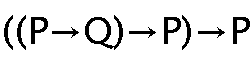
\includegraphics[scale=0.5]{pics/peirce0}}\qquad
\fbox{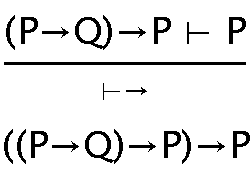
\includegraphics[scale=0.5]{pics/peirce1}}\qquad
\fbox{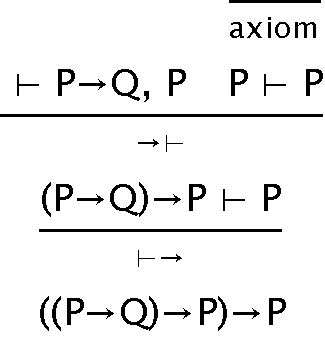
\includegraphics[scale=0.5]{pics/peirce2}}\qquad
\fbox{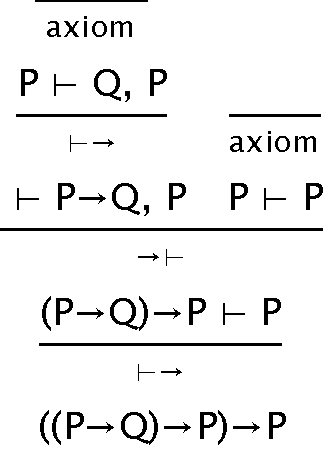
\includegraphics[scale=0.5]{pics/peirce3}}\qquad
\caption{Proof of Peirce's law by double-clicking in the multiple-conclusion sequent calculus}
\label{fig:peirce}
\end{figure}


\section{A very small example}

\Figref{peirce} shows the progress of a proof of Pierce's law in this encoding (which, you can see, is resoundingly classical).
